\chapter{ ANALYSE DES BESOINS}

\section{Les besoins fonctionnels}

        \subsection{Communication avec le serveur}
        Pour éviter toute intrusion d'une personne extérieure et garantir la sécurité des utilisateurs, un serveur a été mis en place par le groupe 1. Ce dernier garantit la vérification de l'identité des utilisateurs, donc tout utilisateur doit pour faire partie du réseau disposer d'une invitation valide qui va lui permettre de s'inscrire.  Ce serveur enregistre tous les utilisateurs, il contient donc les pseudonymes, les numéros de téléphones et les certificats.
        Notre application communique avec ce serveur lors de l'inscription d'un utilisateur(utilisation d'un lien d'inscription valide), lorsque ce dernier souhaite se connecter à l'application(vérification de l'adéquation pseudonyme et mot de passe) mais aussi quand il souhaite envoyer une image à un autre utilisateur(récupérer une liste de numéros par lesquelles doivent transiter les paquets).
            
        
        \subsection{Authentification}
        Lors de son inscription, un utilisateur doit fournir son numéro de téléphone, choisir un identifiant et un mot de passe. La page d'accueil de l'application offre donc une interface pour permettre l'enregistrement de ces informations.
        Lors de la première demande de connexion, une communication est établie avec le serveur pour vérifier les informations de l'utilisateur afin de lui permettre d'accéder aux services fournis par l'application.
        
        \subsection{Ajouter un contact}
        Une fois connecté, comme dans tout réseau social, on a souvent des échanges et des interactions avec les mêmes personnes. Donc pour faciliter les communications entre les utilisateurs, un service d'ajout de contact a été implémenté. Ainsi tout utilisateur peut ajouter des contacts et donc avoir une liste d'amis avec lesquels interagir. Lors de l'envoi d'une image à un ami cette fonctionnalité n'empêche pas que les paquets sur le réseau transitent par les téléphones d'autres utilisateurs (authentifiés par le serveur) qu'on ne connaîtrait pas. Pour enregistrer un contact il faut fournir un nom et son identifiant.
        

        \subsection{Sélection d'un destinataire}
        
        Lorsqu'un utilisateur veut envoyer une image à un autre, il peut sélectionner ce dernier dans sa liste de contacts enregistrés.
       
        
        
        \subsection{Sélection de l'image à envoyer}
        Depuis la page d'envoi, l'utilisateur sélectionne l'image à envoyer dans la galerie d'images de son téléphone  en cliquant sur un bouton prévu à cet effet. %%indexer ici la capture d'ecran de la page d'envoie 
        
        Pour cela, l'utilisateur doit au préalable autoriser l'application à accéder à l'espace de stockage des images de son téléphone.
        
        \subsection{Envoi de l'image}
        Pour optimiser la taille des paquets, après avoir cliqué sur le bouton d'envoi, l'image sélectionnée est d'abord compressée, ce qui permet de faciliter son découpage en fragment d'images (voir ~\ref{decoupage} ). Chaque fragment est concaténé à d'autres champs pour former l'entête du paquet SMS(~\ref{epSMS}),  puis envoyé à des noeuds intermédiaires, qui à leurs tours le renvoient à d'autres, ainsi de suite. Le paquet se promène jusqu'à ce qu'il arrive à destination ou jusqu'à ce que son temps de vie (TTL: time to live) expire.
        
       
        %\subsection{Gestion de l'équilibre carbone}
        %pas gérée pour le moment
            

\section{Les besoins non fonctionnels}
        
        \subsection{Portabilité sur les différentes versions d'Android}
            L'application développée est compatible avec un maximum de terminaux android. Nous avons donc choisi une version minimale requise d'android permettant la plus large compatibilité possible. Il apparaît que rendre l'application compatible avec les systèmes android 4.4 et ses versions ultérieures, permet à environ 98\%
            des terminaux android sur le marché, d'être compatible avec notre application, ce qui est nettement suffisant. Notre application est donc compatible avec les systèmes android 4.4 et ultérieur.

        
        \subsection{Compatibilité avec les autres parties du projet global}
            Le projet Evernet étant divisé en trois sous-projets, notre application est en mesure de s'intégrer avec les deux autres sous-projets afin que le projet global puisse être fonctionnel. Elle est donc en capacité d'utiliser les services de sécurité offerts par le serveur fourni par le groupe 1. Le groupe 3 devant retracer le parcours des paquets sur le réseau, notre entête contient suffisamment d'informations afin que ceci soit possible. Des informations comme la source initiale, la destination finale sont indispensables au groupe 3 et sont donc présentes dans l'entête de nos paquets.  
        
        \subsection{Simplicité d'utilisation}
            
            La simplicité d'utilisation est essentiel pour l'expérience utilisateur. Une interface simple et ergonomique est nécessaire au bon développement de l'application. Une interface trop complexe conduira à une non-utilisation de l'application par les publics cibles qui se tourneront vers des solutions plus simples. Pour ce faire un respect des règles d'Interface Homme-Machine est nécessaire. Ces règles posent un cadre qui permet au développeur de réaliser l'interface la plus ergonomique et simple possible, pour que l'application soit plus simple et agréable à utiliser.
            
              \subsection{Environnement de développement}
            L'application est conçue pour fonctionner sous le système d'exploitation mobile android. Ce qui nécessite d'utiliser un environnement de développement approprié.
            Il a donc été choisi d'utiliser Android Studio. 
            
            \subsection{Langage de programmation}
            Java est le langage de programmation qui a été retenu pour ce projet. Ce dernier étant recommandé par le client, est compatible avec Android Studio. Le langage Kotlin est également compatible avec Android Studio. Seul Java est connu par tous les membres de notre groupe.
\section{Contraintes}
Ce projet amène différentes contraintes techniques qui sont :
\\

\begin{itemize}
\item [•]{Application du Network coding}
            
            La pierre angulaire de ce projet est l'utilisation du \textbf{Network Coding}. Cette façon de gérer les paquets SMS circulant sur le réseau permet d'optimiser le trafic, et d'augmenter la sécurité.
            Lorsque plusieurs paquets ayant la même destination arrivent sur un noeud du réseau, les données que ces paquets portent sont combinées pour former une seule donnée. On peut ainsi envoyer un seul paquet contenant les données combinées et la façon dont les données sont combinées.
            On réduit ainsi le nombre de paquets nécessaires pour transmettre l'information, on allège donc la charge sur le réseau.
            De plus la combinaison des données améliore la sécurité du réseau en chiffrant les données. La manière de combiner les données induit un chiffrement de ces données. On doit donc disposer de la formule de combinaison et d'un ou plusieurs paquets propres à chaque combinaison pour pouvoir déchiffrer les données.
            
            \begin{figure}[H]
                \centering
                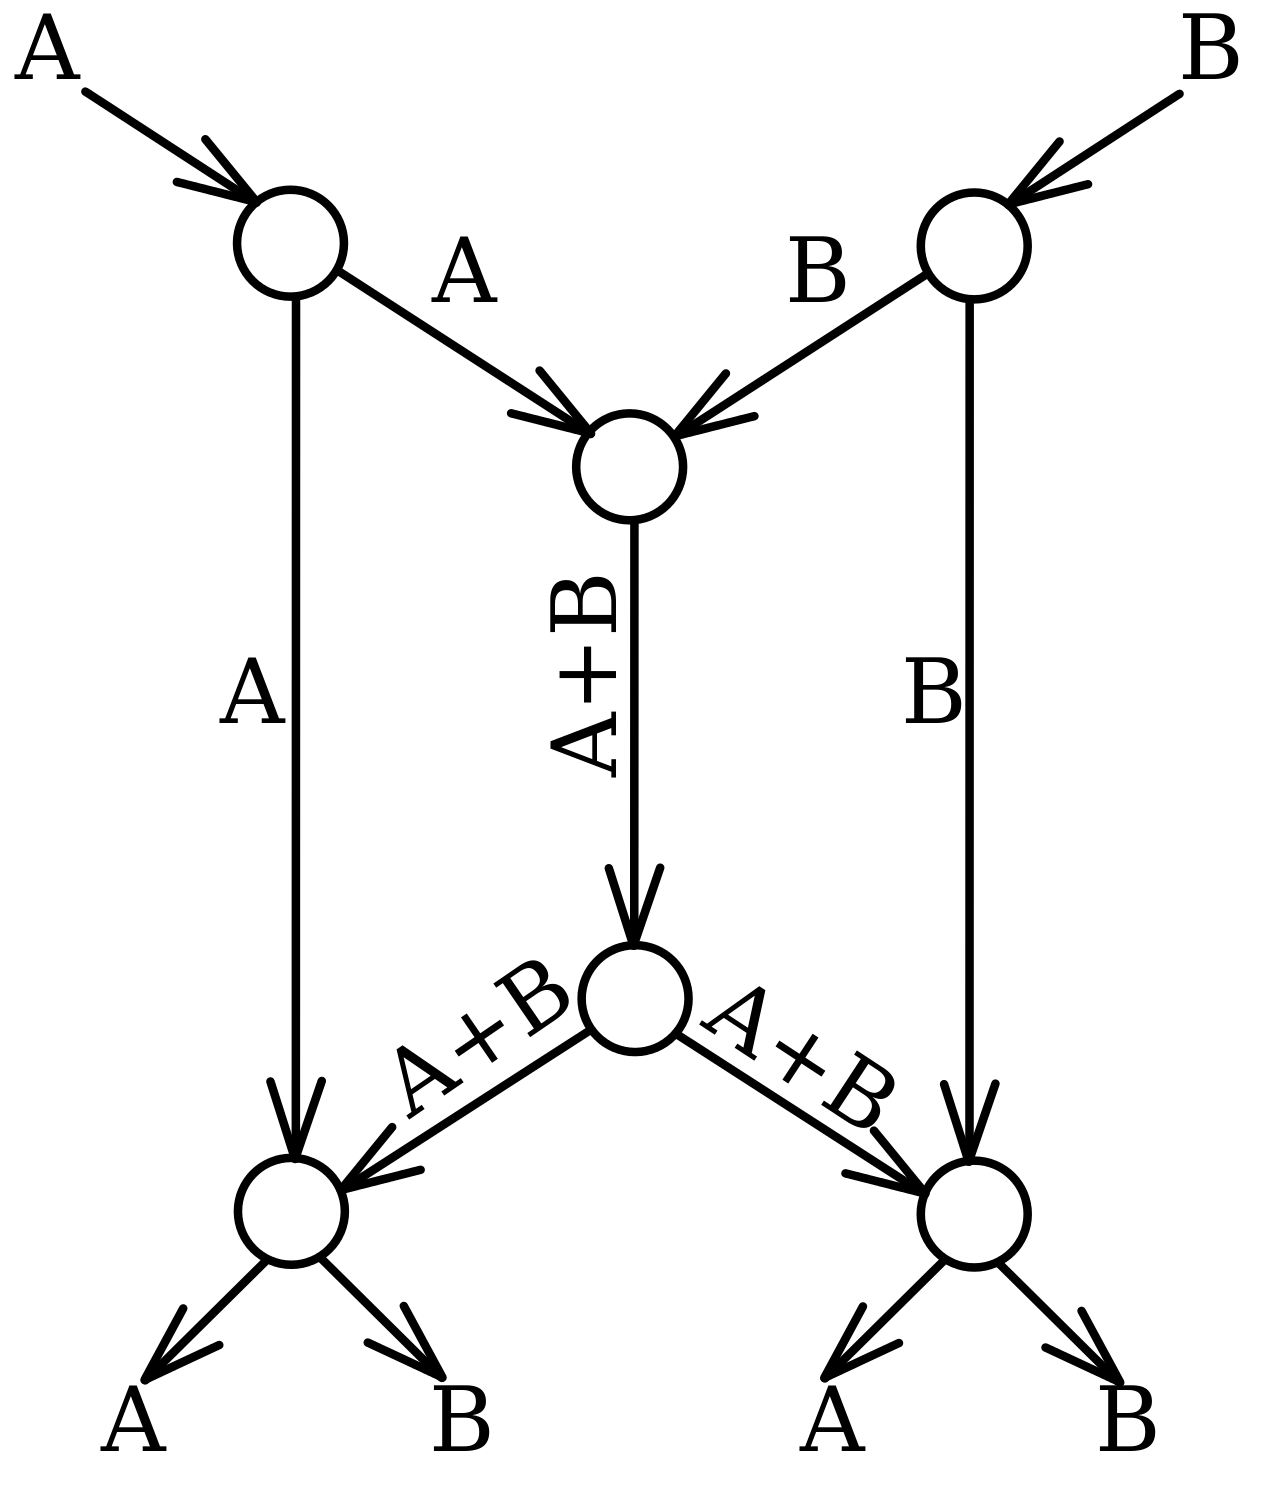
\includegraphics[scale=0.15]{images/Butterfly_network.svg.png}
                \caption{Exemple de Network Coding}
                \label{fig:exemple_Network_Coding}
            \end{figure}
            
            Comme on le voit ci-dessus, les paquets \textbf{A} et \textbf{B} sont combinés pour former un paquet \textbf{A}+\textbf{B}. Ce paquet \textbf{A}+\textbf{B} n'est déchiffrable dans ce cas-ci, seulement si on dispose du paquet \textbf{A} ou du paquet \textbf{B}.
            On retrouvera par exemple le paquet \textbf{B} en faisant : \\ (\textbf{A}+\textbf{B}) - \textbf{A} = \textbf{B}.
            \\
            
    \item [•] Absence de connectivité Internet :
    \\
    le système n'utilisera que les SMS
    \\
    
    \item [•] Equilibrage de la charge énergétique et de l'empreinte carbone :
    \\
    les différents slots de l'image passeront par différents mobiles intermédiaires
    de membres du réseau social
    \\
    
    \item [•]  Confidentialité :
    \\
     les numéros de mobiles des participants doivent rester confidentiels.
     Un serveur central est donc utilisé pour gérer l'association
     pseudonyme-numéro
     \\
     \item [•] Environnement non sécurisé avec risques de perte de messages
        et d'injection de faux messages :
        \\
        une PKI est mise en place pour assurer l'authentification des participants
     \\
     
     \item [•] Optimisation de la bande passante :
     \\
    la technique du Network Coding sera utilisée

\end{itemize}
